\documentclass[11pt, a4paper]{article} %or article has only section and below, book and report also have chapter: http://texblog.org/2007/07/09/documentclassbook-report-article-or-letter/

\usepackage[utf8]{inputenc}  

\usepackage{caption}    		

\usepackage{etoolbox}    
\usepackage[bottom]{footmisc}  
\usepackage{graphicx}       
\usepackage[hidelinks]{hyperref}		
%\usepackage{listings}
\usepackage{lscape}
\usepackage{euler}     
\usepackage[margin=1in]{geometry}

%------------------------------------------------------------------------------------------------------
%------- text size settings --------------
%\setlength{\textwidth}{16cm}% 
%\setlength{\textheight}{25cm} %23 
%(these values were used to fill the page more fully and thus reduce the number of pages!)
%\setlength{\topmargin}{-1.5cm} %0
%\setlength{\footskip}{1cm} %
%\setlength{\hoffset}{0cm} %
%\setlength{\oddsidemargin}{1cm}%
%\setlength{\evensidemargin}{-.5cm}%
%\setlength{\parskip}{0cm} % Abstand zwischen Absätzen
% ----------------------------------------------------------------
%\renewcommand{\textfraction}{0.1} % allows more space to graphics in float
%\renewcommand{\topfraction}{0.85}
%\renewcommand{\bottomfraction}{0.65}
%\renewcommand{\floatpagefraction}{0.70}


\frenchspacing %http://texwelt.de/wissen/fragen/1154/was-ist-french-spacing-was-macht-frenchspacing
%------------------------------------------------------------------------------------------------------
%------------------------------------------------------------------------------------------------------

\usepackage{Sweave}
\begin{document}
\Sconcordance{concordance:sweave_document_TB.tex:sweave_document_TB.Rnw:%
<<<<<<< Updated upstream
1 39 1 1 0 22 1 1 8 4 1 1 7 1 2 9 1 2 2 4 1 1 4 1 1 1 4 20 1}
=======
1 39 1 1 0 24 1 1 7 1 2 6 1 1 4 1 2 3 1}
>>>>>>> Stashed changes



\title{Appendix}

\author{Torfinn and Carolina}

\maketitle

%------------------------------------------------------------------------------------------------------
%------------------------------------------------------------------------------------------------------


\section{Introduction}%------------------------------------------------------------------------------------------------------

We created an appendix of meta-analysis paper. To be able to visualize the output, we used an example dataset taken from Gibson et al. 2011.
The appendix includes forest plots, funnel plots and tables visualizing the results created in the meta-analysis.
\bigskip


%The dataset to be working with should be named ``data.sub''. The conducted analysis using the function rma from the metafor pacakge should be renamed as such: rma of a random effects model should be named ``rma.RE'' and an rma of a fixed effects model should be named ``rma.FE'' in order for the automatisation to work. IF a meta-regression has been conducted, it should be called ``rma.RE.meta'' or ``rma.FE.meta'' respectively. Other than that, the metafor package in R needs to be installed.  






\begin{figure}
\captionsetup{width=0.6\textwidth}
\centering
\includegraphics[width=1\textwidth]{sweave_document_TB-forest}
\caption{Forest plot of a random effects model. The study and its respectice effect size (ES) is shown. The weight given to the study (\%) as well as the effect size (ES) [+- 95\% CI] are shown.}
\label{fig:forestplot}
\end{figure}

The forest plot shows 

%Table with values for ES, SE (ES),pES, CI, I2, Egger value and fasil-sage number. An rma with various moderators can be loaded into this table as well. 


\bigskip




% latex table generated in R 3.1.1 by xtable 1.7-4 package
% Tue Nov 25 17:05:25 2014
\begin{table}[ht]
\centering
\caption{Results of the meta-analysis.ES = Effect Size, Q = Test for residual heterogeneity, $I^2$ = residual heterogeneity, Egger's test and the fails-safe number for publication bias testing.} 
{\footnotesize
\scalebox{0.9}{
\begin{tabular}{rccccccccccc}
  \hline
 & {ES} & \parbox{1cm}{SE of ES} & CI (lb) & CI (ub) & P(ES) & Q & P(Q) & I^2 & Egger & P(Egger) & FSN \\ 
  \hline
Meta-Analysis & -0.28 & 0.12 & -0.52 & -0.04 & 0.02 & 47.05 & 0.12 & 27.22 & -0.44 & 0.66 & 77.00 \\ 
   \hline
\end{tabular}
}
}
\end{table}

\bigskip

%Table of the meta-regression. In this case only for one moderator. 


% latex table generated in R 3.1.1 by xtable 1.7-4 package
% Tue Nov 25 17:05:25 2014
\begin{table}[ht]
\centering
\caption{Results of the meta-regression (mixed-effects model). The model results are shown taking a moderator into account and displaying the coefficients. Results for the whole model are displayed as Q = Test for residual heterogeneity, $I^2$ = residual heterogeneity and QM = Test of Moderators.} 
{\footnotesize
\scalebox{0.9}{
\begin{tabular}{rccccc|ccccc}
  \hline
 & {ES} & \parbox{1cm}{SE of ES} & CI (lb) & CI (ub) & P(ES) & Q & P(Q) & I^2 & QM & P(QM) \\ 
  \hline
intrcpt & -0.353 & 0.766 & -1.85 & 1.15 & 0.645 & 22.7 & 0.54 & 0.000493 & 24.4 & 0.0278 \\ 
  continentAS & -0.377 & 0.423 & -1.21 & 0.452 & 0.373 &  &  &  &  &  \\ 
  continentCA & -0.0485 & 0.61 & -1.24 & 1.15 & 0.937 &  &  &  &  &  \\ 
  continentSA & -0.627 & 0.375 & -1.36 & 0.108 & 0.0945 &  &  &  &  &  \\ 
  metricric & 0.119 & 0.254 & -0.38 & 0.617 & 0.641 &  &  &  &  &  \\ 
  disturbanceagf & 0.331 & 0.745 & -1.13 & 1.79 & 0.657 &  &  &  &  &  \\ 
  disturbanceagr & 0.701 & 0.936 & -1.13 & 2.54 & 0.454 &  &  &  &  &  \\ 
  disturbancebur & 0.723 & 0.731 & -0.709 & 2.15 & 0.322 &  &  &  &  &  \\ 
  disturbanceoth & 0.728 & 0.903 & -1.04 &  2.5 & 0.42 &  &  &  &  &  \\ 
  disturbancepas & -0.0589 & 0.979 & -1.98 & 1.86 & 0.952 &  &  &  &  &  \\ 
  disturbancepla & -0.203 & 0.868 & -1.9 &  1.5 & 0.815 &  &  &  &  &  \\ 
  disturbancesec & 0.399 & 0.723 & -1.02 & 1.82 & 0.581 &  &  &  &  &  \\ 
  disturbancesel & 0.796 & 0.691 & -0.559 & 2.15 & 0.25 &  &  &  &  &  \\ 
  disturbanceshd & -0.908 & 0.783 & -2.44 & 0.626 & 0.246 &  &  &  &  &  \\ 
   \hline
\end{tabular}
}
}
\end{table}




%<< echo=FALSE, eval=TRUE >>=
%sens.RE = leave1out(rma.RE)
%if ((length(which(sens.RE$I2 < 25))) > 0) {
%  (which(sens.RE$I2 < 25))
%} else {
%      (which((rma.RE$I2 - sens.RE$I2) > 4))}
%@

\Sexpr{if (rma.RE$pval < 0.05) {
  if (length(which(sens.RE$pval > 0.05) > 0)) 
    { paste0("The leave-one out analysis shows that the following study(ies) lead to insignificance of the meta analysis:", (which(sens.RE$pval > 0.05))) 
  } else {
    paste0("The leave-one out analysis shows that no left-out studies yielding non-significance. This means that the studies ")
  }
} else {
  if (length(which((sens.RE$pval < 0.05) > 0))) { paste0(The leave-one out analysis shows that study ", which(sens.RE$pval < 0.05))  
  } else {
    paste("The leave-one out analysis shows that no left-out studies yield significance of the original meta analysis.")
  }}}

To assess possible publication bias, funnel plots can be used for visualization purposes.When publication bias is absent, the plot should have a symmetrical shape of a funnel around the mean effect size. This is because the precision of the estimation of effect size, should increase with sample size (smaller standard error). 


\begin{figure}
\captionsetup{width=0.6\textwidth}
\centering
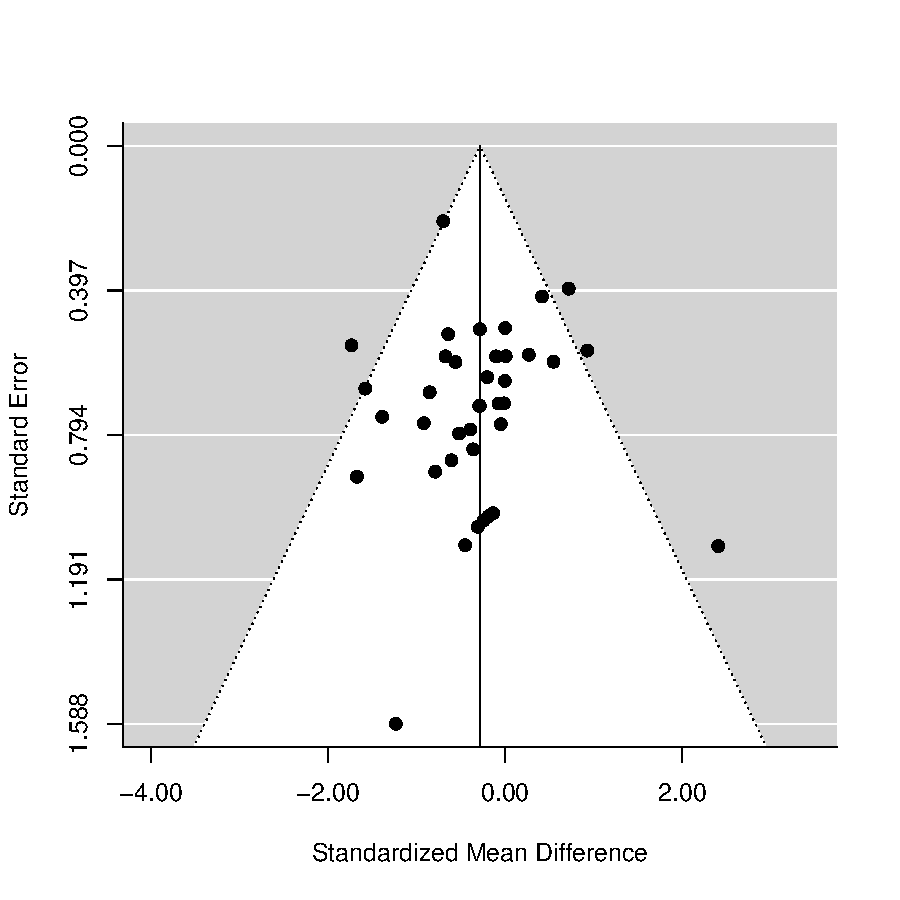
\includegraphics[width=0.7\textwidth]{sweave_document_TB-funnelplot}
\caption{Funnel plot of random effects model displaying possible publication bias. The true ES is displayed by the solid verical line.}
\end{figure}



\begin{figure}
\captionsetup{width=0.6\textwidth}
\centering
\includegraphics[width=1\textwidth]{sweave_document_TB-diagnostics}
\caption{Diagnostic plots for diagnostics of meta analysis. Standardized residual plot, normal Q-Q plot, Baujat heterogeneity plot and Galbrath's radial plot are shown.}
\label{fig:diagnostics}
\end{figure}


\begin{figure}
\captionsetup{width=0.6\textwidth}
\centering
\includegraphics[width=1\textwidth]{sweave_document_TB-forestreg}
\caption{Forest plot of a random effects regression model. The column on the left represents the study. The weighted percentage is shown as well as the effect size (ES) [+- 95\% CI]}
\label{fig:forestplotreg}
\end{figure}


  



% latex table generated in R 3.1.1 by xtable 1.7-4 package
% Tue Nov 25 17:05:27 2014
\begin{table}[ht]
\centering
\caption{This output of the sensitivity analysis (leave1out analysis) shows the results of the meta analysis when a study is left out. This table reports the top most influential studies on the effect size, sorted by absolute change in effect size. The Left-out study indicates which study is left out to produce the results. ES = effectsize, SE = Standard error, CI =  95 percent confidence interval, P(ES) = p-value of estimate, Q = Test for residual heterogeneity, P(Q) = p-value of heterogenity value, $I^2$ = residual heterogeneity} 
{\footnotesize
\scalebox{0.9}{
\begin{tabular}{cccccccccc}
  \hline
\parbox{1.05cm}{left-out study} & {ES} & ES change & \parbox{1cm}{SE of ES} & CI (lb) & CI (ub) & P(ES) & Q & P(Q) & I^2 \\ 
  \hline
  15 & -0.342 & -0.0589 & 0.117 & -0.572 & -0.113 & 0.0035 & 39.6 & 0.311 & 17.5 \\ 
     7 & -0.232 & 0.0517 & 0.118 & -0.463 & -0.000631 & 0.0494 & 40.1 & 0.293 & 20.1 \\ 
    35 & -0.324 & -0.0409 & 0.121 & -0.56 & -0.088 & 0.00715 &   42 & 0.227 & 23.1 \\ 
    11 & -0.244 & 0.0389 & 0.127 & -0.493 & 0.00424 & 0.054 & 42.6 & 0.208 & 22.9 \\ 
   \hline
\end{tabular}
}
}
\end{table}



\end{document}
